% !TeX spellcheck = en_US
\documentclass[letterpaper,12pt,twoside]{report}
\usepackage{fancyhdr}
\usepackage{fullpage}
\usepackage{tikz}
\usepackage{amsmath}

\begin{document}
	\pagestyle{fancy}
	\fancyhf{}
	\fancyhead[L]{Day 21}
	\fancyhead[R]{\textit{The Calendar Project}}
	\fancyfoot[L]{Citations Involved: none}
	
	% Problem
	\paragraph{Problem}
	\begin{quote}
		\textsf{There exist many points inside a
			triangle such that segments can be drawn
			from the point to the sides of the triangle
			(not at the vertices) so that the three
			resulting quadrilaterals have equal areas.
			There is only one point inside a triangle
			such that the segments drawn to the
			vertices create three quadrilaterals of
			equal area. How is the point determined?}
	\end{quote}
	
	% Graphics
	\begin{center}
		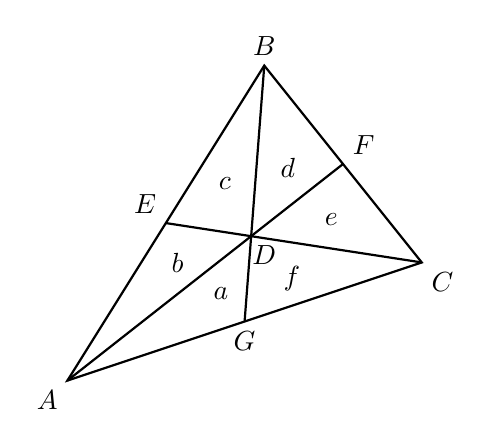
\begin{tikzpicture}[scale=0.5]
		\draw[thick] (-5,-5) -- (0,3) -- (4,-2) -- cycle;
		\draw[thick] (0,3) -- (-0.5,-3.5);
		\draw[thick] (4,-2) -- (-2.5,-1);
		\draw[thick] (-5,-5) -- (2,0.5);
		
		\node[below left] at (-5,-5) {$A$};
		\node[above] at (0,3) {$B$};
		\node[below right] at (4,-2) {$C$};
		\node at (0,-1.8) {$D$};
		\node[above left] at (-2.5,-1) {$E$};
		\node[above right] at (2,0.5) {$F$};
		\node[below] at (-0.5, -3.5) {$G$};
		
		\node at (-1.1,-2.8) {$a$};
		\node at (-2.2,-2) {$b$};
		\node at (-1,0) {$c$};
		\node at (0.6,0.4) {$d$};
		\node at (1.7,-0.9) {$e$};
		\node at (0.7,-2.4) {$f$};
		
		\end{tikzpicture}
	\end{center}
	
	% Reasoning
	\paragraph{Reasoning}
	\begin{quotation}
		
		Draw $\overline{BG}$, $\overline{AF}$, and $\overline{CE}$ as medians of $\triangle ABC$. Name their point of coincidence $D$; since the three medians of a triangle coincide at its centroid, $D$ is the centroid of $\triangle ABC$.
		
		The definition for a median of a triangle is a segment whose endpoints are a vertex of the triangle and the midpoint of the opposite side (3). As such, $G$ is the midpoint of $\overline{AC}$, $F$ is the midpoint of $\overline{BC}$, and $E$ is the midpoint of $\overline{AB}$; thus $G$ is equidistant from $A$ and $C$, $E$ is equidistant from $A$ and $B$, and $F$ is equidistant from $B$ and $C$ by definition, and therefore $AG=GC$, $AE=EB$, and $BF=FC$. The definition of a triangle's altitude is a perpendicular segment from a vertex to the \textbf{line containing the opposite side} (4); Since $\overline{AG}$ and $\overline{GC}$ are contained in the same line ($\overleftrightarrow{AC}$), and since $\triangle ABG$ and $\triangle CBG$ share $B$ as the vertex opposite that line, the altitudes of $\triangle ABG$ and $\triangle CBG$ refer to the same segment and therefore have the same length. The formula for the area of a triangle is $\frac{1}{2}bh$ where $b$ is the length of its base and $h$ is the length of its height, or its altitude (4); since the lengths of the bases of $\triangle ABG$ and $\triangle CBG$ ($AG$ and $GC$) are equal, and since they share the same altitude, $\triangle ABG$ and $\triangle CBG$ have the same area. Similarly, $\triangle BCE$ and $\triangle ACE$ have the same area, $\triangle BAF$ and $\triangle CAF$ have the same area, $\triangle ADG$ and $\triangle CDG$ have the same area, $\triangle BDF$ and $\triangle CDF$ have the same area, and $\triangle BDE$ and $\triangle ADE$ have the same area.
				
		Let $a$, $b$, $c$, $d$, $e$, and $f$ refer to the areas of $\triangle ADG$, $\triangle ADE$, $\triangle BDE$, $\triangle BDF$, $\triangle CDF$, and $\triangle CDG$ respectively (as shown above). By the Angle Addition Postulate (1), $[\triangle ABG]=a+b+c$, $[\triangle CBG]=d+e+f$, $[\triangle BCE]=c+d+e$, $[\triangle ACE]=a+b+f$, $[\triangle BAF]=b+c+d$, and $[\triangle CAF]=a+e+f$. By the Transitive Property, $a+b+c=d+e+f, c+d+e=a+b+f$, and $b+c+d=a+e+f$. Using these symbols, the previously determined equalities in area can be expressed as $a=f, d=e$, and $b=c$. After respective substitution with regard to the previously determined equalities in area, $a+b+c=d+e+a$, $c+d+e=a+c+f$, and $b+b+d=a+d+a \Rightarrow b+c=d+e=e+e=a+f, b+b=a+a \Rightarrow 2b=2a \Rightarrow a=b=c=f, b+b=e+e=d+e=a+a \Rightarrow 2b=2e=2a \Rightarrow a=b=c=f=e=d$.
		
		The three quadrilaterals created by the radians are $ABDC$, $ADBC$, and $ADCB$. By the Area Addition Postulate (5), $[ABDC]=a+b+c+f, [ADBC]=a+d+e+f, $ and $[ADCB]=b+c+d+e$. Since $a=b=c=d=e=f$, $[ABDC]=a+a+a+a$, $[ADBC]=a+a+a+a$, and $[ADCB]=a+a+a+a \Rightarrow [ABDC]=[ADBC]=[ADCB]$. This confirms that for any triangle, the three quadrilaterals created by segments drawn from the centroid to the vertices of $\triangle ABC$ have equal area. Since it is given that there is only one point in a triangle that accomplishes this, the $\boxed{\text{centroid}}$ is the solution to this problem.
	\end{quotation}
	
	\paragraph{External References}
	
	\begin{enumerate}
		\item Textbook Ch. 1, Pg. 22: Angle Addition Postulate
		\item Textbook Ch. 1, Pg. 36: Perimeter and Area of a Triangle
		\item Textbook Ch. 5, Pg. 314: Definition of a Median of a Triangle
		\item Textbook Ch. 5, Pg. 316: Definition of an Altitude of a Triangle
		\item Textbook Ch. 9, Pg. 589: Area Addition Postulate
	\end{enumerate}
	
\end{document}